% =======================================================================
% =                                                                     =
% =======================================================================
% -----------------------------------------------------------------------
% - Author:     Chaua Queirolo                                          -
% - Version:    001                                                     -
% -----------------------------------------------------------------------
\documentclass[a4paper,11pt]{article}    

% =======================================================================
% PACKAGES
% =======================================================================

% Language support
\usepackage[brazil]{babel}
\usepackage[utf8]{inputenc}
\usepackage[T1]{fontenc}
\usepackage{ae,aecompl}

% Configuration
\usepackage{url}
\usepackage{enumerate}
\usepackage{color}
\usepackage[svgnames,table]{xcolor}
\usepackage[margin=2cm,includefoot]{geometry}

% Tabular
\usepackage{multirow}
\usepackage{multicol}

% Images
\usepackage{graphicx}
\usepackage{caption}
\usepackage[scriptsize]{subfigure}
\usepackage{epstopdf}
\usepackage{float}% http://ctan.org/pkg/{multicol,lipsum,graphicx,float}

% Math
\usepackage{mdwtab}	% bug rowcolor
\usepackage{amssymb}
\usepackage{amsmath}
\usepackage{footnote}

% References
\usepackage[sort,nocompress]{cite}

% =======================================================================
% VARIABLES
% =======================================================================

% Space between the lines in a table
\renewcommand{\arraystretch}{1.3}

% Define a new column type
\newcolumntype{x}[1]{>{\raggedright\hspace{0pt}}p{#1}}%

% Controle das Margens
\sloppy
\tolerance=9999999

% Espaço entre colunas
\setlength{\columnsep}{.9cm}


% Configuration
\usepackage{lipsum}
\usepackage{blindtext}

% =======================================================================
% HEADER
% =======================================================================

\title{K-Means}
\author{Felipe Eduardo Lopes\\E-mail: {\tt felipe\_lopes@outlook.com}}
\date{}

\newenvironment{Figure}
  {\par\medskip\noindent\minipage{\linewidth}}
    {\endminipage\par\medskip}

% =======================================================================
% DOCUMENT
% =======================================================================
\begin{document}
\graphicspath{ {} }
\maketitle

\begin{multicols}{2}

\section{Introdução}
O objetivo do algoritmo K-Means é fornecer uma classificação de informações de acordo com os dados fornecidos. Esta classificação, é baseada em análises e comparações entre os valores. O algoritmo vai, automaticamente fornecer uma classificação sem a necessidade de nenhuma supervisão humana, ou seja, sem precisar de pré-classificação. Por causa desta característica, o K-Means é considerado como um algoritmo de mineração de dados não supervisionado.\cite{ref:chibelushi2003}

\section{Descrição do Algoritmo}
O algoritmo tem como objetivo fazer o agrupamento de elementos em classes, o número de classes é o mesmo número de centroides. Podem existir diversos centroides, que deverão ser gerados aleatoriamente. O Número de Centroides é definido pela constante K. 

\section{Métodos}
Para mostrar o funcionamento do K-means, vamos separar seu funcionamento em alguns passos:\\

\subsubsection{Centroides}
O número de centroides no algoritmo é definido pela constante K, ou seja se o K = 2 então teremos dois centroides. As posições dos centroides devem ser geradas aleatoriamente em uma posição do plano.

\subsubsection{Matriz de Distâncias}
Após os centroides serem gerados, devemos calcular a distância de cada ponto do plano com os centroides. Para o cálculo, normalmente é utilizado o algoritmo euclidiano.

\subsubsection{Classificação dos prontos}
Cada ponto do plano deve ser classificado, é atribuído ao centroide o ponto mais próximo a ele. Caso tenhamos N centroides, teremos N classes com os pontos mais próximos a ele.

\subsubsection{Mover os centroides}
Após a primeira classificação dos pontos para seu centroide, é necessário recalcular o cento da massa do centroide, com o objetivo de deixar a classificação mais refinada possível.  O novo valor dos centroides é calculado fazendo-se a média de cada atributo de todos os pontos que pertencem a esta classe. Caso exista alteração em sua posição deve-se voltar para o passo 3.0.2. Quando o centroide não se mover mais, teremos a classificação final dos pontos.

\section{Exemplos de aplicações}
As aplicações para o algoritmo são diversas, pois com ele podemos buscar padrões difíceis de serem detectados pelo seres humanos. Como por exemplo, classificação de clientes em classes, cliente ouro, bronze e prata. Como demonstrado na Figura 1, o algoritmo foi capaz de classificar elementos em um plano 3D em duas classes.

\begin{Figure}
	\centering 
	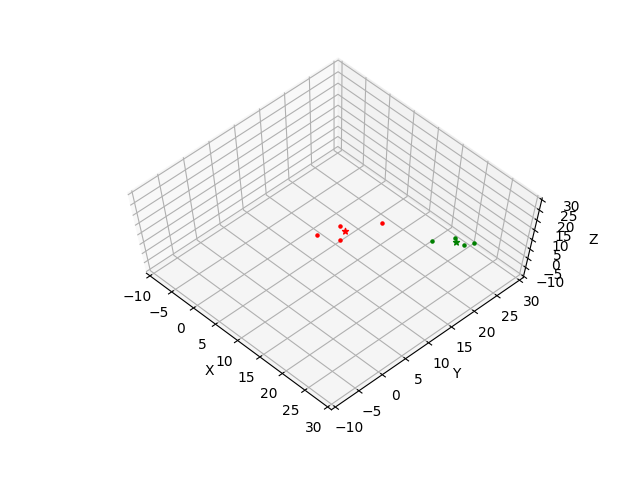
\includegraphics[width=8cm, height=7cm]{figura1}
	\captionof{figure}[]{Agrupamento de elementos em um espaço 3D. Fonte: Próprio Autor}
	\label{medium}
\end{Figure}


\bibliographystyle{plain}
\bibliography{referencias}

\end{multicols}
\end{document}

